\documentclass{article}
\usepackage[utf8]{inputenc}
\usepackage[english]{babel}
\usepackage{graphicx}
\usepackage{enumerate}
\usepackage{float}
\graphicspath{ {} }
\usepackage{mathtools}
\usepackage{amsmath, amsthm, amssymb, amsfonts}
\usepackage{caption}
\usepackage{fancyhdr}
\pagestyle{fancy}
\fancyhf{}
\rhead{Ty Darnell}
\lhead{Homework 10}
\allowdisplaybreaks
% For derivatives
\newcommand{\deriv}[1]{\frac{\mathrm{d}}{\mathrm{d}x} (#1)}

% For partial derivatives
\newcommand{\pderiv}[2]{\frac{\partial}{\partial #1} (#2)}

% Integral dx
\newcommand{\dx}{\mathrm{d}x}
\begin{document}
\begin{flushleft}
\chead{Problem 1-3}
\section*{Problem 1}
\begin{align*}
\text{Let } U&= X/Y \text{ and } V=Y\\
\text{Then } X&=UV, \quad Y=V\\
\text{ where } &X \text{ and } Y \text{ are independent } \chi^2 \text{ r.v.s with m and n degrees of freedom respectively}\\
\text{WTS: } U& \sim F_{m,n} \text{ that is:}\\
f_U(u)&=\dfrac{m}{n}\dfrac{\Gamma(\dfrac{m+n}{2})(\dfrac{m}{n}u)^{m/2-1}}{\Gamma(m/2)\Gamma(n/2)(1+u(m/n))^{(m+n)/2}} \ u>0\\
\text{Let } c&=m/2 \text{ and } d=n/2\\
f_X(x)&=\dfrac{1}{\Gamma(c)2^c}x^{c-1}e^{-x/2} \ x>0\\
f_Y(y)&=\dfrac{1}{\Gamma(d)2^d}y^{d-1}e^{-y/2} \ y>0\\
f_{XY}(x,y)&=\left(\dfrac{1}{\Gamma(c)2^c}x^{c-1}e^{-x/2}\right) \left(\dfrac{1}{\Gamma(d)2^d}y^{d-1}e^{-y/2}\right)\\
&=\dfrac{1}{\Gamma(c)\Gamma(d)2^{c+d}}x^{c-1}y^{d-1}e^{-x/2}e^{-y/2} \ x,y>0\\
J(u,v)&=
\begin{bmatrix}
\dfrac{\partial x}{\partial u} & 
\dfrac{\partial x}{\partial v}\\ 
\dfrac{\partial y}{\partial u} &
\dfrac{\partial y}{\partial v} 
\end{bmatrix}
= \begin{bmatrix}
v & u \\
0 & 1
\end{bmatrix}
=v\\
f_{UV}(u,v)&=\dfrac{1}{\Gamma(c)\Gamma(d)2^{c+d}}(uv)^{c-1}v^{d-1}e^{-(uv+v)/2}|v| \ u,v>0\\
f_U(u)&=\int_{0}^{\infty}f_{UV}(u,v) \ dv=\int_{0}^{\infty}\dfrac{v}{\Gamma(c)\Gamma(d)2^{c+d}}(uv)^{c-1}v^{d-1}e^{-(uv+v)/2} \ dv\\
&=\int_{0}^{\infty}\dfrac{u^{c-1}}{\Gamma(c)\Gamma(d)2^{c+d}}v^{c+d-1}e^{-v(u+1)/2} \ dv\\
f_U(u)&=\dfrac{u^{c-1}}{\Gamma(c)\Gamma(d)2^{c+d}}\int_{0}^{\infty}v^{c+d-1}e^{-v(u+1)/2} \ dv\\
\text{Let } z&=\dfrac{v(u+1)}{2}\\
dz&=\dfrac{u+1}{2} \ dv\\
dv&=\dfrac{2}{u+1} \ dz\\
f_U(u)&=\dfrac{u^{c-1}}{\Gamma(c)\Gamma(d)2^{c+d}}\int_{0}^{\infty}\dfrac{2z}{u+1}^{c+d-1}e^{-z} \dfrac{2}{u+1} \ dz\\
&=\left(\dfrac{2}{u+1}\right)^{c+d}\dfrac{u^{c-1}}{\Gamma(c)\Gamma(d)2^{c+d}}\int_{0}^{\infty}z^{c+d-1}e^{-z} \ dz\\
&=\left(\dfrac{2}{u+1}\right)^{c+d}\dfrac{u^{c-1}}{\Gamma(c)\Gamma(d)2^{c+d}}\Gamma(c+d)\\
&=\dfrac{\Gamma(c+d)}{\Gamma(c)\Gamma(d)}\dfrac{u^{c-1}}{(u+1)^{c+d}}\\
f_{(n/m)(UV)(u)}&=\dfrac{m}{n}f_U(\dfrac{m}{n}u)\\
&=\dfrac{m}{n}\dfrac{\Gamma(\dfrac{m+n}{2})}{\Gamma(m/2)\Gamma(n/2)}\dfrac{((m/n)u)^{m/2-1}}{((m/n)u+1)^{(m+n)/2}}\\
\text{Thus } &\dfrac{X/m}{Y/n} \sim F(m,n)
\end{align*}
\section*{Problem 2}
\begin{align*}
f_{x}(\boldmath{X})&= \begin{cases} \dfrac{2}{2e-5} x_1^2x_2e^{x_1x_2x_3} \quad & 0<x_1,x_2,x_3<1\\
0 \quad & \text{otherwise}
\end{cases}\\
\text{Let } Y_1&=X_1*X_2*X_3\\
Y_2&=X_1\\
Y_3&=X_2\\
\text{Then } X_1&=Y_2\\
X_2&=Y_3\\
X_3&=\dfrac{Y_1}{Y_2Y_3}\\
J(y_1,y_2,y_3)&=
\begin{bmatrix}
\dfrac{\partial x_1}{\partial y_1} & 
\dfrac{\partial x_2}{\partial y_1}&
\dfrac{\partial x_3}{\partial y_1}\\ 
\dfrac{\partial x_1}{\partial y_2} & 
\dfrac{\partial x_2}{\partial y_2}&
\dfrac{\partial x_3}{\partial y_2}\\
\dfrac{\partial x_1}{\partial y_3} & 
\dfrac{\partial x_2}{\partial y_3}&
\dfrac{\partial x_3}{\partial y_3}
\end{bmatrix}
=\begin{bmatrix}
0& 0 & 1/(y_2y_3)\\
1 & 0& -(y_1/y_3)y_1^{-2}\\
0&1&-(y_1/y_2)y_3^{-2}
\end{bmatrix}\\
J(y_1,y_2,y_3)&=\dfrac{1}{y_2y_3}\\
f_y(\boldmath{Y})&=\dfrac{2}{2e-5}y_2^2y_3e^{y_1}\bigg|\dfrac{1}{y_2y_3}\bigg|\\
f_y(\boldmath{Y})&=\begin{cases}
\dfrac{2}{2e-5}y_2e^{y_1} \quad & 0<y<1\\
0 \quad & \text{otherwise}
\end{cases}\\
0&< y_1< y_2< 1\\
\dfrac{y_1}{y_2}&< y_3< 1\\
f_y(y_1)&=\int_{y_1}^{1}\int_{y_1/y_2}^{1}\dfrac{2}{2e-5}y_2e^{y_1} \ dy_3 dy_2\\
&=\dfrac{2}{2e-5}\int_{y_1}^{1}y_2e^{y_1}-y_1e^{y_1}\ dy_2\\
&=\dfrac{2}{2e-5}(1/2)e^{y_1}(1-2y_1+y_1^2)\\
&=\dfrac{1}{2e-5}e^{y_1}(1-y_1)^2\\
f_y(y_1)&=\begin{cases}
\dfrac{1}{2e-5}e^{y_1}(1-y_1)^2 \quad & 0<y_1<1\\
0 \quad & \text{otherwise}
\end{cases}\\
\text{Thus the pdf of }& X_1*X_2*X_3 \text{ is } f_y(y_1)
\end{align*}
\section*{Problem 3}
\begin{align*}
f(x)&=e^{-x}\\
f_y&=e^{-y}\\
f_{X,Y}(x,y)&=e^{-x}e^{-y}=e^{-(x+y)} \ x,y>0\\
\text{Let } U&=X+Y \text{ and } V=X\\
X&=V \quad Y=U-V\\
J(u,v)&=\begin{bmatrix}
0 & 1\\
1 & -1
\end{bmatrix}=-1\\
f_{U,V}(u,v)&=f_{X,Y}(v,u-v)=e^{-(v+u-v)}=e^{-u}, \ 0<v<u<\infty\\
f_{V|U=c}(v)&=\dfrac{f_{U,V}(c,v)}{f_U(c)}=\dfrac{e^{-c}}{ce^{-c}}=\dfrac{1}{c}, \ 0<v<c\\
&\text{Which is distributed as } U(0,c)
\end{align*}
\pagebreak
\section*{Problem 4}
\chead{Problems 4-6}
\begin{enumerate}[(a)]
\item
\begin{align*}
-2&\leq x \leq 4 \quad \text{7 values}\\
x-1&\leq y \leq x+1 \quad \text{3 values}\\
3*7&=21 \text{ possible } (x,y) \text{ pairs}\\
x&\in [-2,4]\\
y&\in [-3,5]\\
p_{X,Y}(x,y)&=\begin{cases}
1/21 &\quad -2\leq x\leq 4 \quad x-1\leq y\leq x+1\\
0 &\quad \text{otherwise}
\end{cases}\\
p_X(x)&=\sum_{y=x-1}^{x+1}p(x,y)=p_X(x)=\begin{cases}
1/7 &\quad -2\leq x \leq 4\\
0 &\quad \text{otherwise}
\end{cases}\\
p_Y(y)&=\sum_{x=-2}^{4}p(x,y)=p_Y(y)=\begin{cases}
1/21 &\quad y=-3,5\\
2/21 &\quad y=-2,4\\
1/7 &\quad -1\leq y \leq 4\\
0 &\quad \text{otherwise}
\end{cases}\\
E[X]&=\sum_{-2}^{4}xp(x)=\dfrac{1}{7}(-2+-1+0+1+2+3+4)=1\\
E[Y]&=\sum_{-3}^{5}yp(y)=\dfrac{1}{21}(-3+5)+\dfrac{2}{21}(-2+4)+\dfrac{1}{7}(-1+0+1+2+3)=1
\end{align*}
\item 
\begin{align*}
100*E[X]+200*E[Y]&=100+200=300\\
\text{Mean of traders profit }&= 300
\end{align*}
\end{enumerate}
\section*{Problem 5}
We have a 2 by 2 square with an area of 4
\begin{enumerate}[(a)]
\item
$X^2+Y^2<1$\\
Since the distribution is continuous this is the same as:\\
$X^2+Y^2\leq 1$\\
Which is a circle with area  $\pi$\\
Since the total area is 4, $P(X^2+Y^2<1)=\dfrac{\pi}{4}$
\item
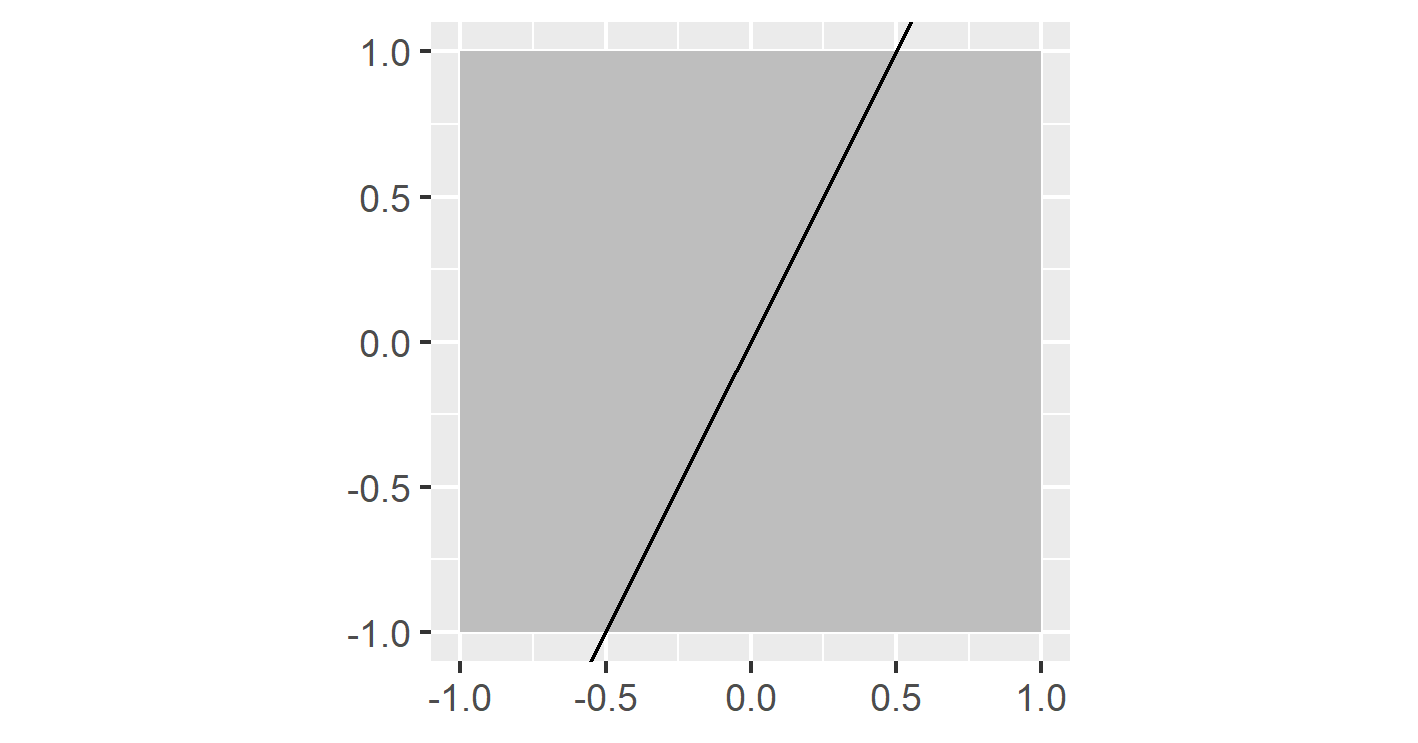
\includegraphics[scale=.7]{plot2.png}\\
$2X+Y>0$\\
$Y<2X$\\
Which is the area below the line $y=2x$\\
Since this line cuts the square in half\\
$P(2X-Y>0)=\dfrac{2}{4}=\dfrac{1}{2}$
\item 
Looking at the plot of $|X+Y|<2$:\\
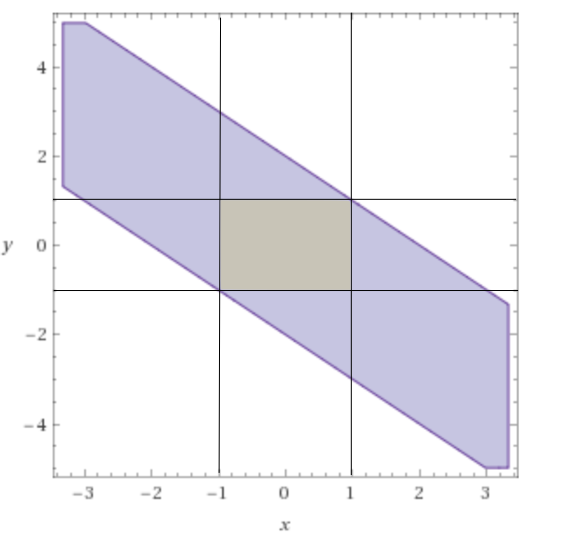
\includegraphics[scale=.4]{abs.png}\\
We can see that this includes the entire rectangle, thus\\
$P(|X+Y|<2)=1$
\end{enumerate}
\pagebreak
\section*{Problem 6}
\begin{enumerate}[(a)]
\item
\begin{align*}
C\int_{0}^{2}\int_{0}^{1}x+2y \ dy \dx&=1\\
C\int_0^2 x+1 \ \dx&=1\\
4C&=1\\
C&=1/4
\end{align*}
\item
\begin{align*}
f_X(x)&=(1/4)\int_{0}^{1}x+2y \ dy\\
&=(1/4)(x+1)\\
f_X(x)&=\begin{cases}
1/4(x+1) \quad & 0<x<2\\
0 \quad & \text{otherwise}
\end{cases}
\end{align*}
\item
\begin{align*}
F_{XY}(x,y)&=\int_{-\infty}^{x}\int_{-\infty}^{y}f(s,t) \ dt \ ds\\
&=(1/4)\int_{0}^{x}\int_{0}^{y}s+2t \ dt \ ds\\
&=(1/8)x^2y+(1/4)xy^2\\
\text{In order to get the} &\text{ complete CDF we must consider the boundaries}\\
\text{setting } x&=2 \text{ we have:}\\
(1/4)y&+(1/2)y^2\\
\text{setting } y&=1 \text{ we have:}\\
(1/8)x^2&+(1/4)x\\
F_{XY}(x,y)&=\begin{cases}
0 \quad & x\leq 0 \text{ or } y\leq 0\\
(1/8)x^2y+(1/4)xy^2 \quad & 0<x<2 \text{ and } 0<y<1\\
(1/2)y+(1/2)y^2 \quad & x\geq 2 \text{ and } 0<y<1\\
(1/8)x^2+(1/4)x \quad & 0 \leq x \leq 2 \text{ and } y\geq 1\\
1 \quad & x \geq 2 \text{ and } y \geq 1
\end{cases}
\end{align*}
\item 
\begin{align*}
f_X(x)&=1/4(x+1) \quad  0<x<2\\
Z=g(x)&=\dfrac{9}{(x+1)^2}\\
\text{When } x&=0 \ z=9\\
\text{When } x&=2 \ z=1\\
1&<z<9\\
X&=3z^{-1/2}\\
\dfrac{dx}{dz}&=(-3/2)z^{-3/2}\\
f_z(z)&=f_x(g^{-1}(z))\bigg|\dfrac{dx}{dz}\bigg|\\
&=(9/8)z^{-2} \quad 1<z<9
\end{align*}
\end{enumerate}
\pagebreak
\section*{Problem 7}
\chead{Problems 7-9}
\begin{enumerate}[(a)]
\item 
\begin{align*}
P(X>\sqrt{Y})&=\int_{0}^{1}\int_{\sqrt{y}}^{1} x+y \ \dx dy\\
&=\int_{0}^{1}1/2+(1/2)y-y^{3/2} \ dy\\
&=1/2+1/4-2/5=7/20
\end{align*}
\item
\begin{align*}
X^2&<Y<X\\
X&<\sqrt{Y} \ X>Y\\
Y&<X<\sqrt{Y}\\
P(X^2<Y<X)&=\int_{0}^{1}\int_{y}^{\sqrt{y}}2x \ \dx dy\\
&=\int_{0}^{1}y-y^2 \ dy\\
&=1/2-1/3=1/6
\end{align*}
\end{enumerate}
\section*{Problem 8}
\begin{align*}
X&\sim U(0,30)\\
Y&\sim U(40,50)\\
30-0&=30  \quad 50-40=10\\
30*10&=300\\
X+Y&<60\\
X&<60-Y\\
P(X+Y<60)&=\int_{40}^{50}\int_{0}^{60-y}\dfrac{1}{300} \ \dx dy\\
&=\dfrac{1}{300}\int_{40}^{50}60-y \ dy\\
&=(1/300)(60*50-50^2/2-60*40+40^2/2)\\
&=150/300=1/2
\end{align*}
\pagebreak
\section*{Problem 9}
\begin{align*}
\text{Given } F_{XY}(x,y)&=F_X(x)F_Y(y)\\
\text{WTS: } \text{For any }  (a,b) \text{ and } (c,d):&
P(a\leq X \leq b, c \leq Y \leq d)=P(a\leq X \leq b) P(c \leq Y \leq d)\\
\text{We know X and Y are independent}&\text{ since the joint cdf equals the marginal cdfs multiplied together}\\
&P(a\leq X \leq b)P(c \leq Y \leq d)\\
&=[P(X\leq b)-P(X\leq a)]*[P(Y\leq d)-P(Y\leq c)]\\
=P(X\leq b)P(Y\leq d)-P(X\leq b)&P(Y\leq c)-P(X\leq a)P(Y\leq d)+P(X\leq a)P(Y\leq c)\\
&=F_X(b)F_Y(d)-F_X(b)F_Y(c)-F_X(a)F_Y(d)+F_X(a)F_Y(c)\\
&=F(b,d)-F(b,c)-F(a,d)+F(a,c)\\
=P(X\leq b, Y \leq d)&-P(X\leq b, Y\leq c)-[P(X\leq a, Y\leq d)-P(X\leq a, Y\leq c)]\\
&=P(X\leq b, c\leq Y \leq d)-P(X\leq a,c\leq Y \leq d)\\
&=P(a\leq X\leq b, c\leq Y\leq d)
\end{align*}
\end{flushleft}
\end{document}
